\documentclass[12pt, letterpaper]{article}

%% these are some different packages that provide different capabilities for text
\usepackage{graphicx}
\usepackage{amsmath}
\usepackage{amssymb}
\usepackage{amsfonts}
\usepackage{listings}
\usepackage{morefloats}
\usepackage{color}
\usepackage{algorithmicx}
\usepackage{algorithm}
\usepackage{algpseudocode}
\usepackage{url}
\usepackage{natbib}
\usepackage[letterpaper]{geometry}
\usepackage{epstopdf}
\usepackage{subfig}
\usepackage{listings}
\usepackage{collectbox}
\usepackage{listings}
\usepackage{blindtext}
\usepackage{tabularx}
\usepackage[toc,page]{appendix}


%%%%%%%%%%%%%%%%%%%%%%%%%%%%%%%%%
%Dr. Hodges editing package
\usepackage{color}
\usepackage{soul}  % provides strikethrough as \st
\newcommand{\brh}[1]{\textcolor{red}{\footnotesize[BRH:\ #1]\ }}
\newcommand{\add}[1]{\textcolor{blue}{#1}}
%%%%%%%%%%%%%%%%%%%%%%%%%%%%%%%%%



\setlength{\topmargin}{-0.5in}
%\setlength{\oddsidemargin}{-0.2in}
%\setlength{\evensidemargin}{-0.2in}
\setlength{\textheight}{9.0in}
\setlength{\textwidth}{6in}


\newcommand{\mybox}{%
    \collectbox{%
        \setlength{\fboxsep}{1pt}%
        \fbox{\BOXCONTENT}%
    }%
}
\definecolor{mygreen}{rgb}{0,0.6,0}


\newcommand{\comment}[1]{\textcolor{red}{\footnotesize[Comment:\ #1]\ }}

%% The default width for eps figures.
\def\epswidth{6.0in}

\title{Simulation Program for River Network (SPRNT) User Guide and Tutorial}

\author{Cheng-Wei Yu \thanks{University of Texas at Austin, Center for Research in Water Resources, yuchanway@utexas.edu}, KyungMin Kim\thanks{University of Texas at Austin, Center for Research in Water Resources, kkim9545@utexas.edu}, Frank Liu \thanks{IBM Research Branch at Austin, frankliu@us.ibm.com} and Ben R. Hodges \thanks{University of Texas at Austin, Center for Research in Water Resources, Associate Professor}}


\date{2016.10.23}
%% end of header information =============================


\begin{document}

\maketitle


\newpage



%%%%%%%%%%
\section*{Introduction}
\label{sec:1}
\indent SPRNT is a one-dimensional hydraulic model developed by Dr. Ben R. Hodges from University of Texas at Austin and Dr. Frank Liu from IBM research branch (Liu and Hodges, 2014). Unlike traditional commercial hydraulic models, SPRNT model is the first hydraulic model that   use the idea from VLSI (very large scale integration) techniques, which were developed for semiconductor circuit analysis and design. This innovation makes SPRNT become the first cross-discipline hydrodynamic model that enable to do the hydrodynamic simulation over a large-scale area (ex. Centennial/Nation-scale). Since SPRNT is a Linux-based model, it does not have fully-feature user interface like other commercial software does. Users will need to change all the parameters/variables/forcings in the code/terminal window.

This user manual will go through every step of executing SPRNT, including installation, data preparation, data preprocess, input file preparation, input file structure, parameter setting, boundary condition setting, commands for running the model and result file structure. There is also a FAQ at the end of this manual, answers for most of common errors/mistakes can be found there. If you are occurring some problems not listed in FAQ section, please feel free to contact Dr. Frank Liu (\url{frankliu@us.ibm.com}), Cheng-Wei Yu (\url{yuchanway@utexas.edu}) or Kyungmin Kim (\url{kkim9545@utexas.edu}) through email. 
\newpage




%%%%%%%%%%
\section{Prerequisite Files}%Before Start}
\label{sec:BS}
Please make sure you have all prerequisite files downloaded.

\subsection{SPRNT Source Code}
\textbf{For Linux system users:}\newline
\\
Linux users can directly download the SPRNT source code from: 
\newline
\newline
\url{https://github.com/frank-y-liu/SPRNT/archive/master.zip} 
\newline
\newline
Or use git command to download the source code. \newline
\begin{lstlisting}[frame=single]
$ git clone https://github.com/frank-y-liu/SPRNT.git
\end{lstlisting}
\textbf{For Mac users:}\newline
\\
Mac users can download the .dmg file from the following link:
\newline
\newline
\url{SPRNT_dmg_file_location} \add{[Maybe put in Frank's Github?]}
\newline
\newline
For Mac users, gfortran package installation is required before the SPRNT installation, please download the appropriate version of gfortran binary package your from the following locaiton: \newline
\newline
\url{https://gcc.gnu.org/wiki/GFortranBinaries#MacOS}
\newline
\newline
[Note: Please try to install the gfortran in the default location (which is -L/usr/local/gfortran/lib), otherwise, user will require modifying the library link path during the installation]


%
%\begin{figure}[H]
%	\centering
%	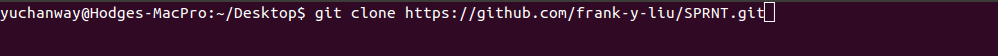
\includegraphics[width = 0.9\textwidth]{figure/how_to_clone_sprnt.png} %
%	\label{fig:process}%
%\end{figure}
%When the cloning is done, you should see the finish message.
%
%\begin{figure}[H]
%	\centering
%	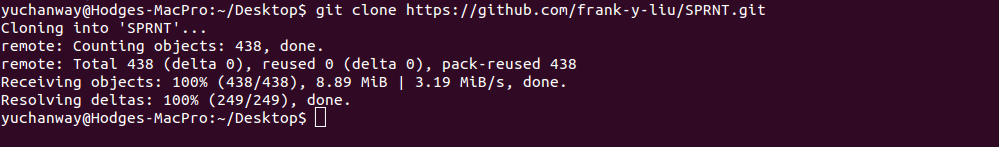
\includegraphics[width = 0.9\textwidth]{figure/git_clone_finish.png} %
%	\label{fig:process}%
%\end{figure}
%
\subsection{Ready to use preprocessor}
\indent The ready-to-use data preprocessor is a program written in C++, users can download it from: \newline
\url{https://github.com/yuchanway/SPRNT_Preprocessor.git}\newline
\newline
or use git command
\begin{lstlisting}[frame=single]
$ git clone https://github.com/yuchanway/SPRNT_Preprocessor.git
\end{lstlisting}
More details about how to use the preprocessor, can be found in \textbf{\emph{Appendix \ref{sec:HtuP}- How to use the Preprocessor}}.
\newpage



%%%%%%
\section{Setting up SPRNT in your machine (for Linux users only)}
\index{How to setup your machine, Linux}


\begin{enumerate}
\item \textbf{./configure in SPRNT directory}\newline
Users need to configure the SPRNT program before executing the installation. Move to /SPRNT/ directory and use the command in the following to configure the SPRNT code:\\

\begin{lstlisting}[frame=single]
$ ./configure
\end{lstlisting}

\item \textbf{Install everything you need indicated as checking \mybox{/compiler/ .... no}} \newline
The configure process will check all the required libraries/packages, users need to install everything listed in the checking.\newline
[Note:g77 may not be required though it says no. gfotran may function as g77, so users will just need to make sure gfortran is installed]

\item \textbf{Install Zlib (zlib-1.2.8)} \newline
For convenience, zlib and hdf5 should be installed in the same folder. Go to the directory where zlib is located,
\begin{lstlisting}[frame=single]
$ ./configure -prefix=/home/ed/local
$ make check install
\end{lstlisting}

\item \textbf{Install HDF5 (hdf5-1.8.14)} \newline
Download the HDF5 source code from: \newline
\url{https://www.hdfgroup.org/downloads/index.html} \newline
Then go to the directory where HDF5 is located and configure the HDF5 source code by using the following commands:
\begin{lstlisting}[frame=single,basicstyle=\footnotesize]
$ ./configure --with-zlib=/home/ed/local -prefix=/home/ed/local
$ make check install
\end{lstlisting}

Related document is also available for reference:\\
\url{https://www.hdfgroup.org/ftp/HDF5/releases/hdf5-1.8.15- patch1/src/unpacked/release_docs/INSTALL}\newline
[Note, this step may take more than 10 mins]

\item \textbf{Install NetCDF4 (netcdf-4.4.0-rc2)} \newline
Users are able to download the NetCDF4 (version netcdf-4.4.0-rc2) from the following link:\newline
\url{https://github.com/Unidata/netcdf-c/releases/tag/v4.4.0-rc2}\newline
After the download is finished, use terminal to go to the directory where NetCDF4 is located, and execute the following command to install the netcdf library.
\begin{lstlisting}[frame=single,basicstyle=\footnotesize]
$ CPPFLAGS=-I/home/ed/local/include LDFLAGS=-L/home/ed/local/lib 
./configure -prefix=/home/ed/local
$ make check install
\end{lstlisting}


\item \textbf{Install UMFPACK}

In this step, some preprocesses are needed:
\begin{enumerate}
\item Install \emph{lapack} library by using the following command:
\begin{lstlisting}[frame=single]
sudo apt-get install libblas-dev liblapack-dev
\end{lstlisting}

\item Install \emph{numpy} and \emph{openblas}, source codes can be found at this website. \\
\url{https://hunseblog.wordpress.com/2014/09/15/installing-numpy-and-openblas}

\item After above steps are finished, users would be able to download and install the \emph{SuiteSparse} package from this website:\\
\url{http://faculty.cse.tamu.edu/davis/suitesparse.html}
\end{enumerate}
After downloading the UMFPACK package, use terminal to go to the directory where UMFPACK is located and executing the following commands:
\begin{lstlisting}[frame=single]
$ make 
$ sudo make install
\end{lstlisting}
After unpackaging, copy and paste the folder to both \mybox{SPRNT/Thirdparty/CMLIB} and \mybox{SPRNT/Thirdparty/UF}

\item \textbf{Install the SPRNT model}

Go to the SPRNT directory and execute the following commands:
\begin{lstlisting}[frame=single]
$ ./configure
$ make dep
$ make
$ make test
$ make install
\end{lstlisting}
\end{enumerate}
\centering
\textbf{Installation finish.}



\newpage
\begin{flushleft}
%%%%%%%%%%%%
\section{Setting up SPRNT in your machine (for Mac users only)}
\index{How to setup your machine, Mac}
\begin{enumerate}

\item \textbf{Mount the dmg file}\newline
Double clicks on the \emph{SPRNT.dmg} file, a hard drive icon will appear on users' desktop. 
\begin{figure}[H]
	\centering
	
\includegraphics[width = 0.45\textwidth]{figure/Mac_installation_1.png} %
	\label{fig:process}%
\end{figure}

\item \textbf{Drag the SPRNT into the Applications folder}\newline
After clicking on the SPRNT hard drive icon, an installation window will pop out. Drag the SPRNT program icon and drop it into the \emph{Applications} folder, like all Mac program installation does.
\begin{figure}[H]
	\centering
	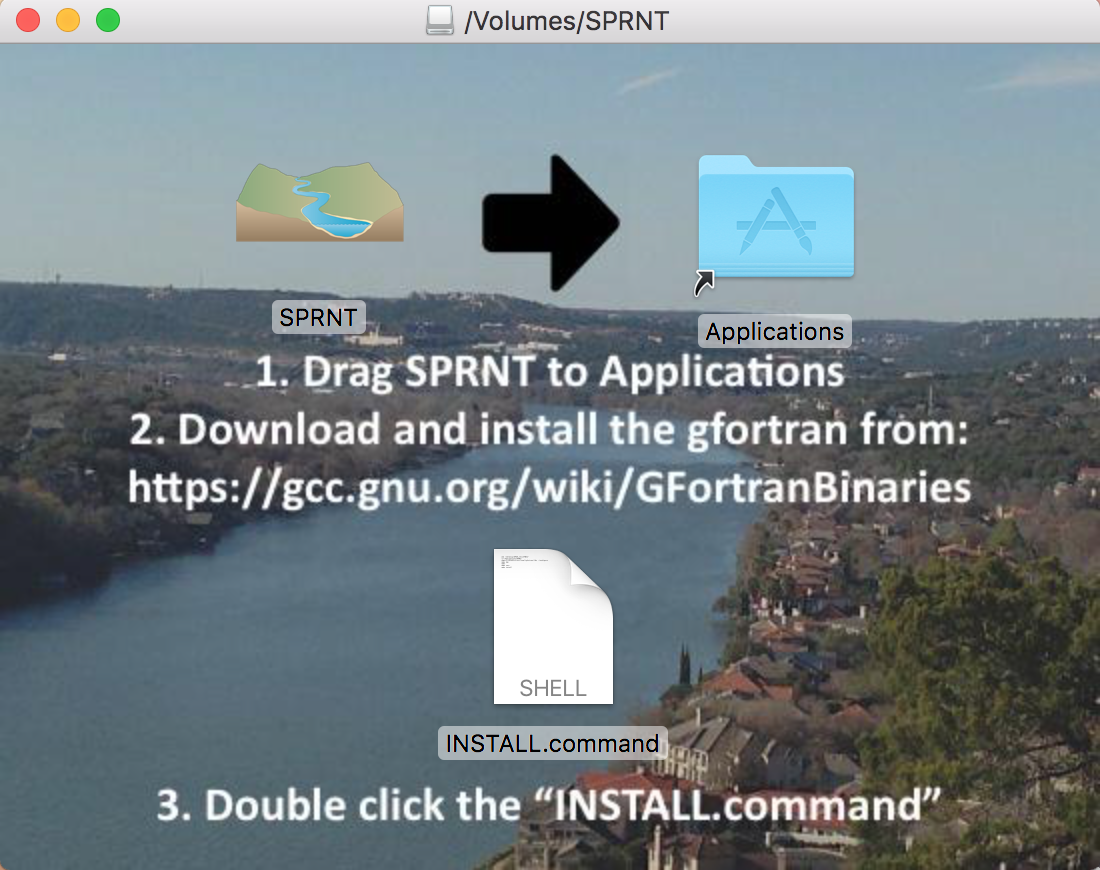
\includegraphics[width = 0.45\textwidth]{figure/Mac_installation_2.png} %
	\label{fig:process}%
\end{figure}

\item \textbf{Install the gfortran library}\newline
Mac users will need to download and install the gfortran package from \url{https://gcc.gnu.org/wiki/GFortranBinaries}. Install the gfortran binary to the default path (which is under \textbf{\emph{/usr/local/}}).\newline
\emph{[NOTE]: If users prefer to install the gfortran binary to other place, the link path in the \emph{INSTALL.command} file need to be modified.}
\item \textbf{Double clicks on \emph{INSTALL.command}}\newline
After the gfortran binary is installed, double clicks on the \emph{INSTALL.command} file. A terminal window will pop out and automatically execute all the required installation commands. 
\end{enumerate}
\centering
\textbf{Installation finish.}
\end{flushleft}





\newpage
%%%%%%%%%%%%
\section{SPRNT Workflow}
The workflow chart in here illustrates all the necessary steps for running a successfully SPRNT simulation. Red denotations in the flowchart represent the order of steps. The detail of each step will be elaborated in the following sections.

\begin{figure}[H]
	\centering
	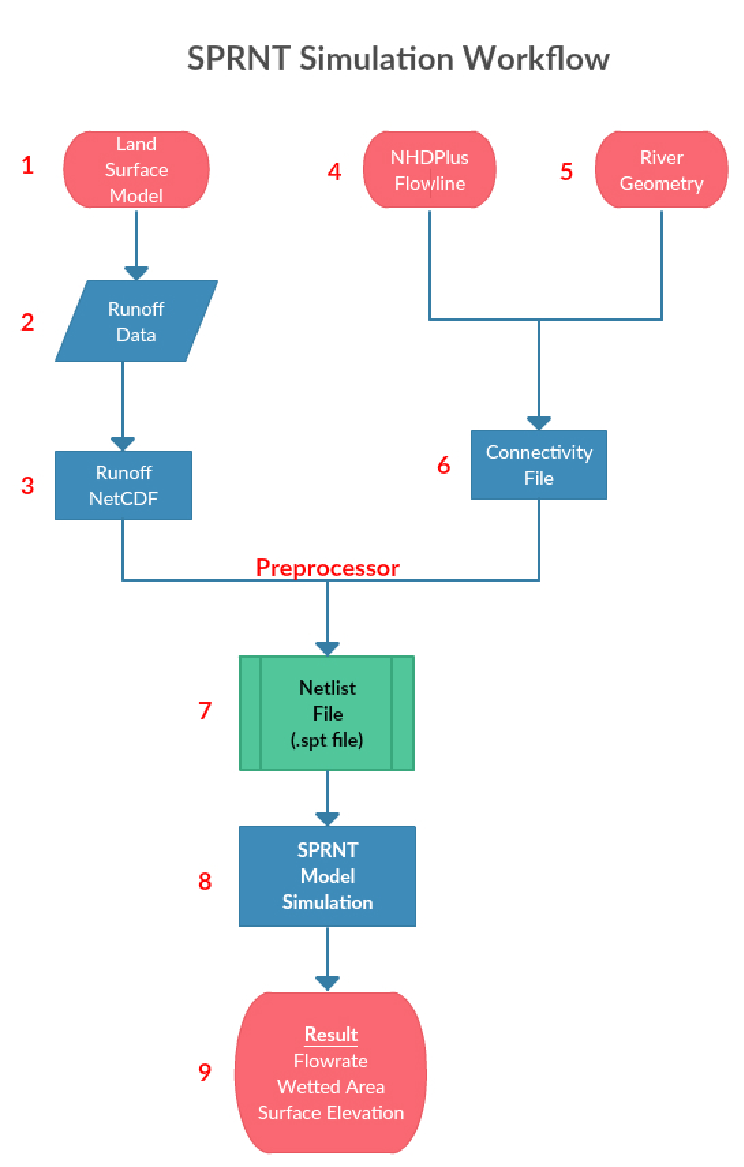
\includegraphics[width = 0.8\textwidth]{figure/Workflow.pdf} %
	\label{fig:process}%
\end{figure}
\newpage

\begin{flushleft} %%Start the left align

\subsection{Land surface model}
In hydraulic/hydrologic modeling, land is an important in component, especially when modeling precipitation and runoff for target river in the study area. Land surface models successfully simulate the land-atmosphere water loop and enable human to predict/approach the precipitation condition in large-scale area. In SPRNT model, we will use the precipitation from land surface models as the lateral flow sources in the model. In here, we made an assumption that the soil in the study area is saturated; so all the effective rainfall from the land surface model will become the river runoff.
Land surface models can be: NOAH, NLDAS 2, JULES...etc. However, please aware of that the choice of land surface model will directly influence the accuracy of the hydraulic simulation result.
\subsection{Runoff data}
In order to successfully run a SPRNT simulation, we need to convert the forcing term to the right format. From the last paragraph, you should get the precipitation data from the land surface mode (normally the unit is mm/hour). Nevertheless, the unit of runoff data for SPRNT to input is m3/sec.


%%%
\subsection{Runoff Netcdf file}
In large-scale hydraulic modeling, sometimes we have to deal with excessive runoff data that can up to several gigabytes. The efficiently way to handle these data is saving them as a NetCDF file.
NetCDF file is a file type commonly used in climatology, meteorology and oceanography applications. It is also a common file type for GIS tools. More information about NetCDF file: \url{https://en.wikipedia.org/wiki/NetCDF}
In SPRNT simulation, the runoff data has to be save into a NetCDF file in the specific format. The example netcdf file in \emph{/SPRNT/Tutorial/ExampleNetcdf/} can be used for users' reference.

%%%
\subsection{NHDPlus flowline}
The SPRNT model uses the NHD Flowline as the frame of the river network. NHD Flowline features can be download from the NHDPlus version 2 website \url{http://www.horizon-systems.com/NHDPlus}.

%%%
\subsection{River geometry}
River geometry is the important input factors in hydraulic routing models. In SPRNT model, there are several types of cross section descriptions are supported for users' choice:

\end{flushleft} %% End the left align



\begin{table}[ht]
\centering
\begin{tabular}{*{2}{m{0.48\textwidth}}}
\hline
\begin{center} Types of cross section description\end{center} & \begin{center}Required Variables \end{center} \\
\hline
\textbf{Trapezoidal}: Two parameters needed to be defined: bottom width and sidewall slope.&\begin{center}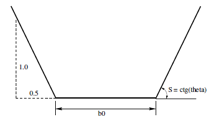
\includegraphics[width = 0.35\textwidth]{figure/Trap.png} \end{center}\\
\hline
\textbf{XY Coordinate system}: Need \textbf{X (station)} and \textbf{Y (elevation)} coordinates to describe the channel shape.& \begin{center}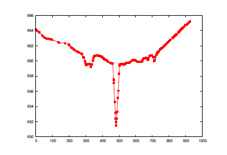
\includegraphics[width = 0.35\textwidth]{figure/XY.png} \end{center}\\
\hline
\textbf{Intrinsic (Hydraulic Propertis)}: Unlike traditional hydraulic models, SPRNT provides a new way to describe channel shape - ``Intrinsic cross section description". In intrinsic description, user will be asked to provide certain hydraulic properties in a certain order: \textbf{A-P-Y-W}. Where A is wetted area, P is wetted perimeter, Y is water depth and W is top width. & \begin{center}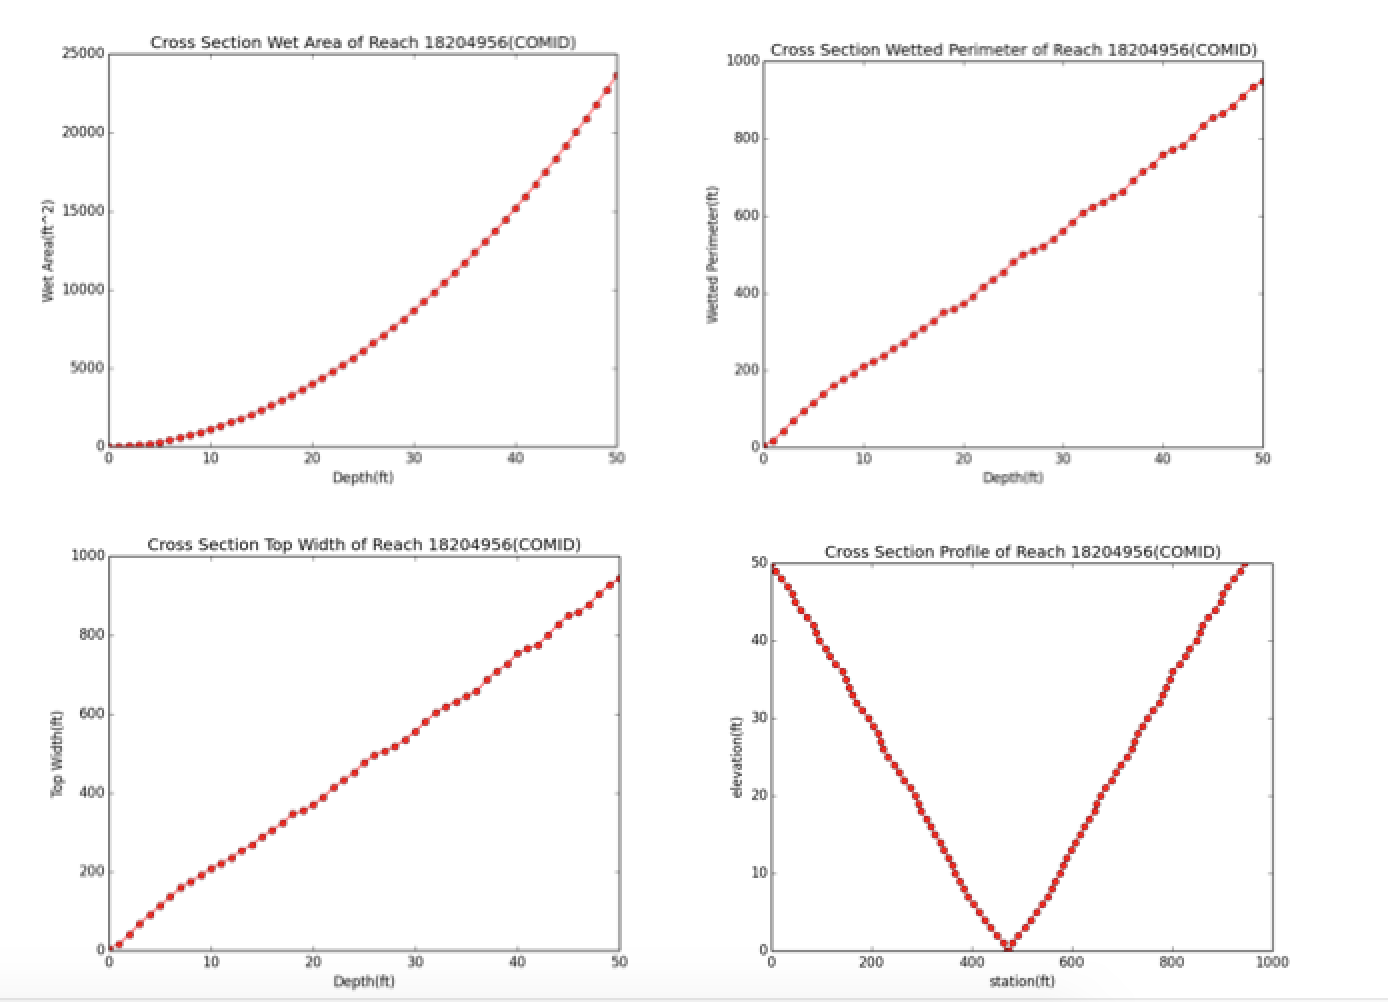
\includegraphics[width = 0.35\textwidth]{figure/HP.png} \end{center}\\
\hline
\end{tabular}
\end{table}


%%%
\subsection{Connectivity file}
\begin{flushleft} %%Start the left align

The figure below illustrates the format of connectivity file. You can find colored columns from each denoted file from NHDPlus data:
\url{http://www.horizon-systems.com/NHDPlus/NHDPlusV2_data.php}
\end{flushleft} %%End the left align

\begin{figure}[H]
	\centering
	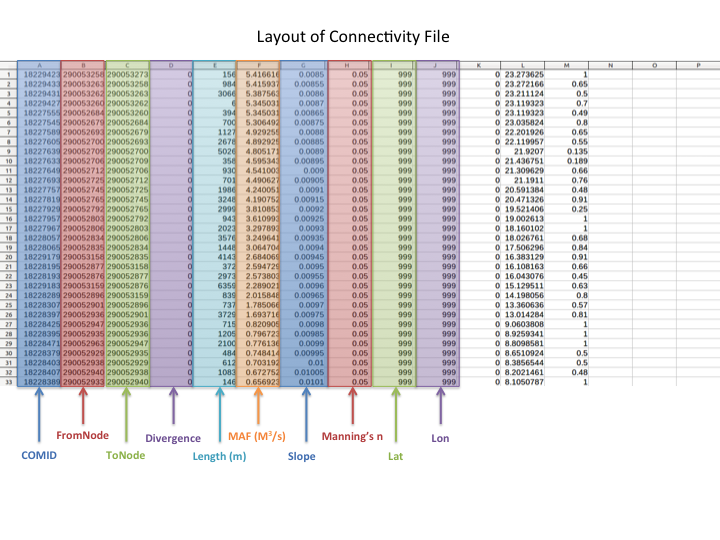
\includegraphics[width = 0.75\textwidth]{figure/LayoutOfConnectovity/Connect_1.png} %
	\label{fig:process}%
\end{figure}
\begin{figure}[H]
	\centering
	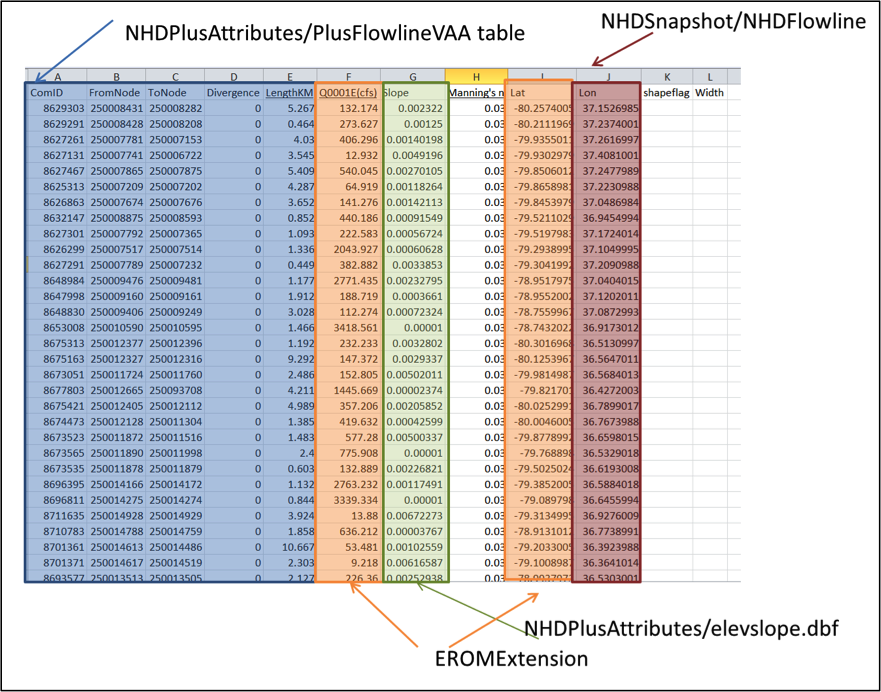
\includegraphics[width = 0.75\textwidth]{figure/NHDPlus.png} %
	\label{fig:process}%
\end{figure}

\begin{flushleft} %%Start the left align
For Manning's n, users will need to specify the value between 0.03 - 0.05 and compare the result with USGS data. Shapeflag is an indicator that represents the types of cross-sections. It can be assigned by three values. (0 : Trapezoidal, 1: XY coordinate and 2: Intrinsic (hydraulic properties) ). When the Shapeflag equals to 0 (trapezoidal description), the following two columns will be Bottom Width and Side Wall Slope. If the Shapeflag was assigned to 1 (XY coordinate), user will need to put the XY data after the Shapeflag column in the order of $X_1$, $Y_1$, $X_2$, $Y_2$...$X_n$, $Y_n$. If user assign the Shapeflag to 2 (Intrinsic description), hydraulic properties should be put in the order of $A_1$, $P_1$, $Y_1$, $W_1$, $A_2$, $P_2$, $Y_2$, $W_2$,......... $A_n$, $P_n$, $Y_n$, $W_n$.
In order to let users to have a better knowledge, two types of connectivity file by using different types of cross section description were illustrated in the following figures:
\end{flushleft} %%End the left align

\begin{figure}[H]
	\centering
	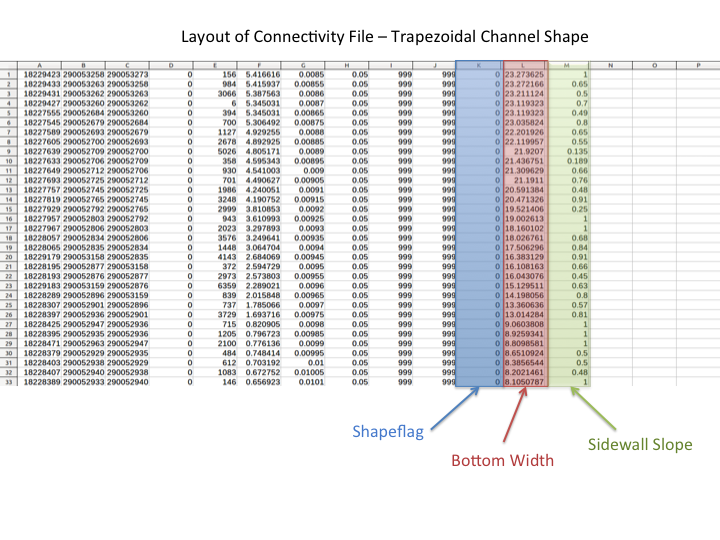
\includegraphics[width = 0.85\textwidth]{figure/LayoutOfConnectovity/Connect_2.png} %
	\label{fig:process}%
\end{figure}
\begin{figure}[H]
	\centering
	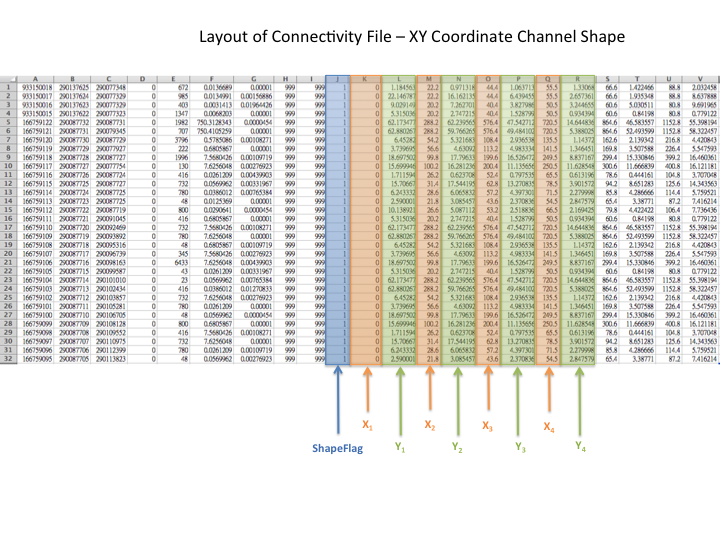
\includegraphics[width = 0.85\textwidth]{figure/LayoutOfConnectovity/Connect_3.png} %
	\label{fig:process}%
\end{figure}
\begin{figure}[H]
	\centering
	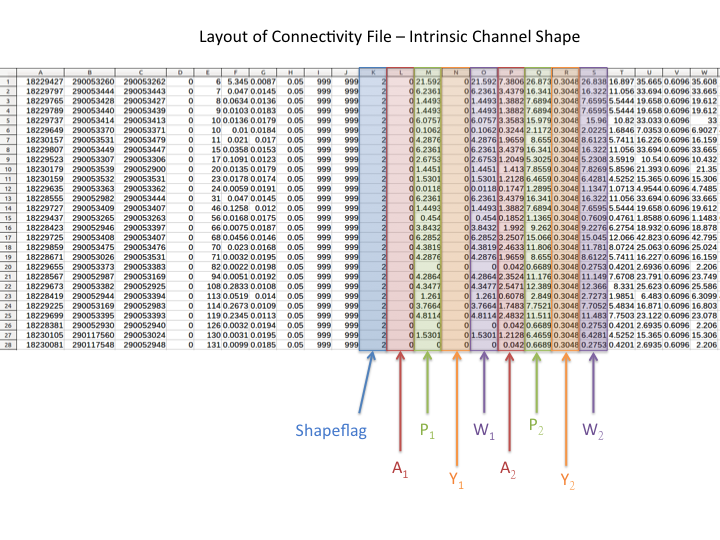
\includegraphics[width = 0.85\textwidth]{figure/LayoutOfConnectovity/Connect_4.png} %
	\label{fig:process}%
\end{figure}

%%%
\subsection{Netlist file (.spt) structure}
\begin{flushleft} %%Start the left align
``Netlist" is an idea that previously used to describe electric circuit topography in computer science. SPRNT model uses the netlist file, which is a text-based file includes a series combinations of ``def" and ``end", to define the channel geometric characteristics, forcing terms, junction contribution ratios and other factors of the simulation.\newline
In here, for users' convenience, we provide a ready-to-use preprocessor(written in C++) for producing netlist files. Please refer to \textbf{``HOW TO USE PREPROCESSOR"} section in appendix for detailed instructions.
The following figure is a small sample of a SPRNT netlist excerpts from Liu and Hodges (2014). For more details on the SPRNT netlist, please refer to the SPRNT users' manual written by Frank Liu (2012). \url{https://github.com/frank-y-liu/SPRNT/blob/master/doc/sprint_manual_rev.pdf}
\end{flushleft} %%End the left align



%%%
\subsection{Execute SPRNT model commands}
\begin{flushleft} %%Start the left align

Once the netlist file was done (the example here is Davis\_Creek.spt), move the netlist file to the bin directory by using the following commands:
\begin{lstlisting}[frame=single]
$ mv FILE_NAME.spt WHERE_YOU_SAVE_SPRNT/SPRNT/bin/
\end{lstlisting}
\begin{figure}[H]
	\centering
	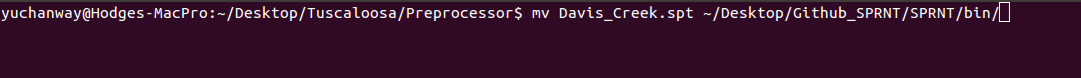
\includegraphics[width = 1.0\textwidth]{figure/mv_to_bin.png} %
	\label{fig:process}%
\end{figure}

Then we have to move to the /SPRNT/bin/ directory by using cd command:

\begin{lstlisting}[frame=single]
$ cd WHERE_YOU_SAVE_SPRNT/SPRNT/bin/
\end{lstlisting}
\begin{figure}[H]
	\centering
	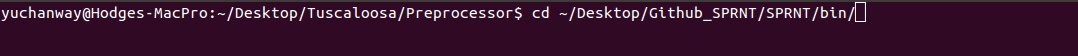
\includegraphics[width = 1.0\textwidth]{figure/cd_to_bin.png} %
	\label{fig:process}%
\end{figure}

Now, your working directory should be /SPRNT/bin. You can use the command ``ls" to list all the visible files in this directory.
The netlist file we just moved to /bin/ directory should be here as well (example file Davis\_Creek.spt)

\begin{lstlisting}[frame=single]
$ ls
\end{lstlisting}
\begin{figure}[H]
	\centering
	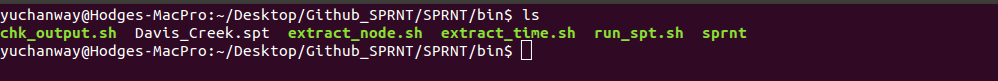
\includegraphics[width = 1.0\textwidth]{figure/ls_in_bin.png} %
	\label{fig:process}%
\end{figure}


To start the SPRNT simulation, we have to execute a shell script called ``run\_spt.sh".
\begin{lstlisting}[frame=single]
$ sh run_spt.sh FILENAME.spt
\end{lstlisting}

\begin{figure}[H]
	\centering
	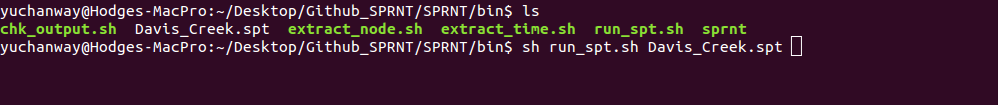
\includegraphics[width = 1.0\textwidth]{figure/runsprnt.png} %
	\label{fig:process}%
\end{figure}

If the SPRNT model is successfully launched, user should see the following message:

\begin{figure}[H]
	\centering
	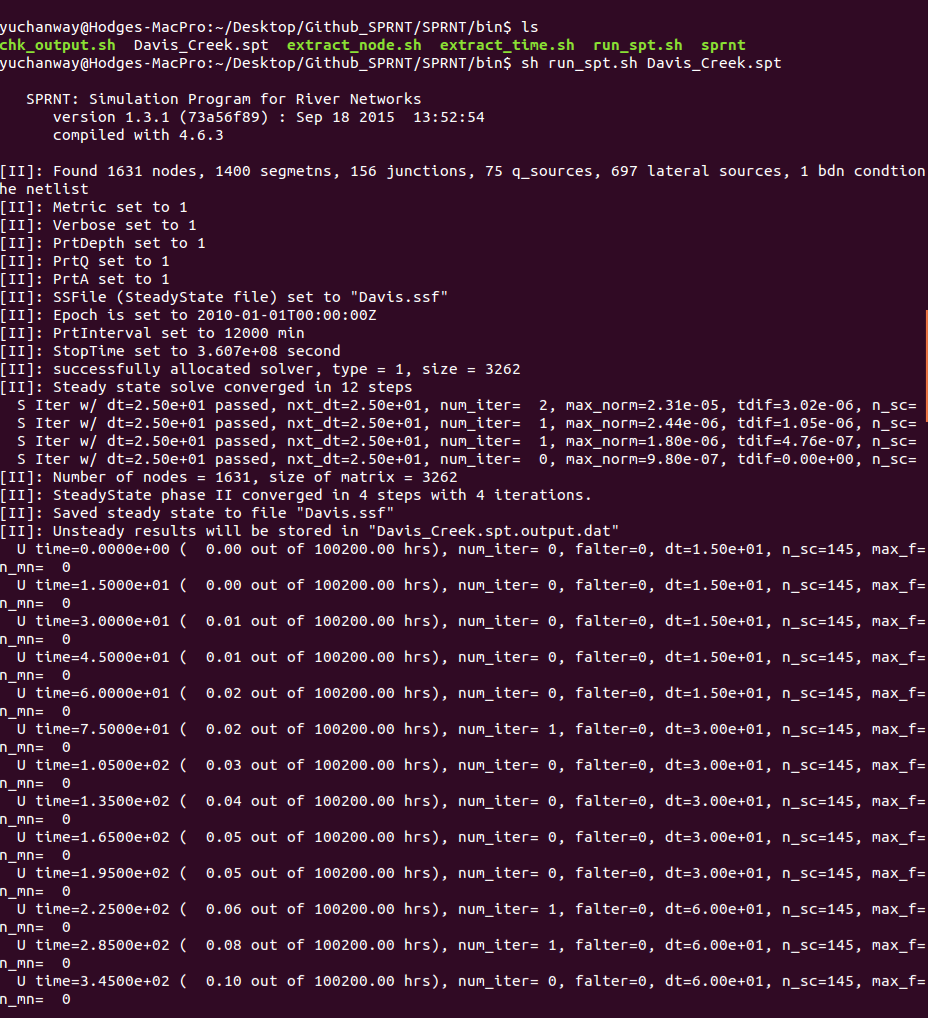
\includegraphics[width = 1.0\textwidth]{figure/startrun.png} %
	\label{fig:process}%
\end{figure}

When the execution is successful, the model will first solve the steady state convergence. After the steady state successfully converges, the steady state result will be saved to a FILENAME.ssf file. The ``.ssf" file was not designed for users to read, so there will After the .ssf file was created, SPRNT model will start solving the unsteady state convergence. The unsteady state results will be saved to a FILENAME.spt.output.dat file.


\begin{figure}[H]
	\centering
	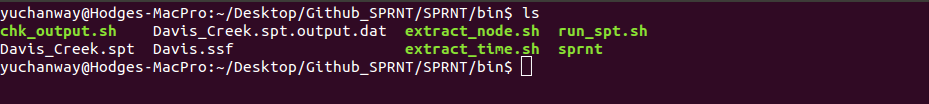
\includegraphics[width = 1.0\textwidth]{figure/outputfile.png} %
	\label{fig:process}%
\end{figure}

%%%
\subsection{Result file structure}
After the unsteady state convergence finished, you will be able to see the file FILENAME.spt.output.dat in your /bin/ directory.
The following screen snapshot is the output file of SPRNT model, named ``Davis\_Creek.spt.output.dat". Basically, the output file is a space-delimitated text-based file, so it can be open by any kind of text reader.

\begin{figure}[H]
	\centering
	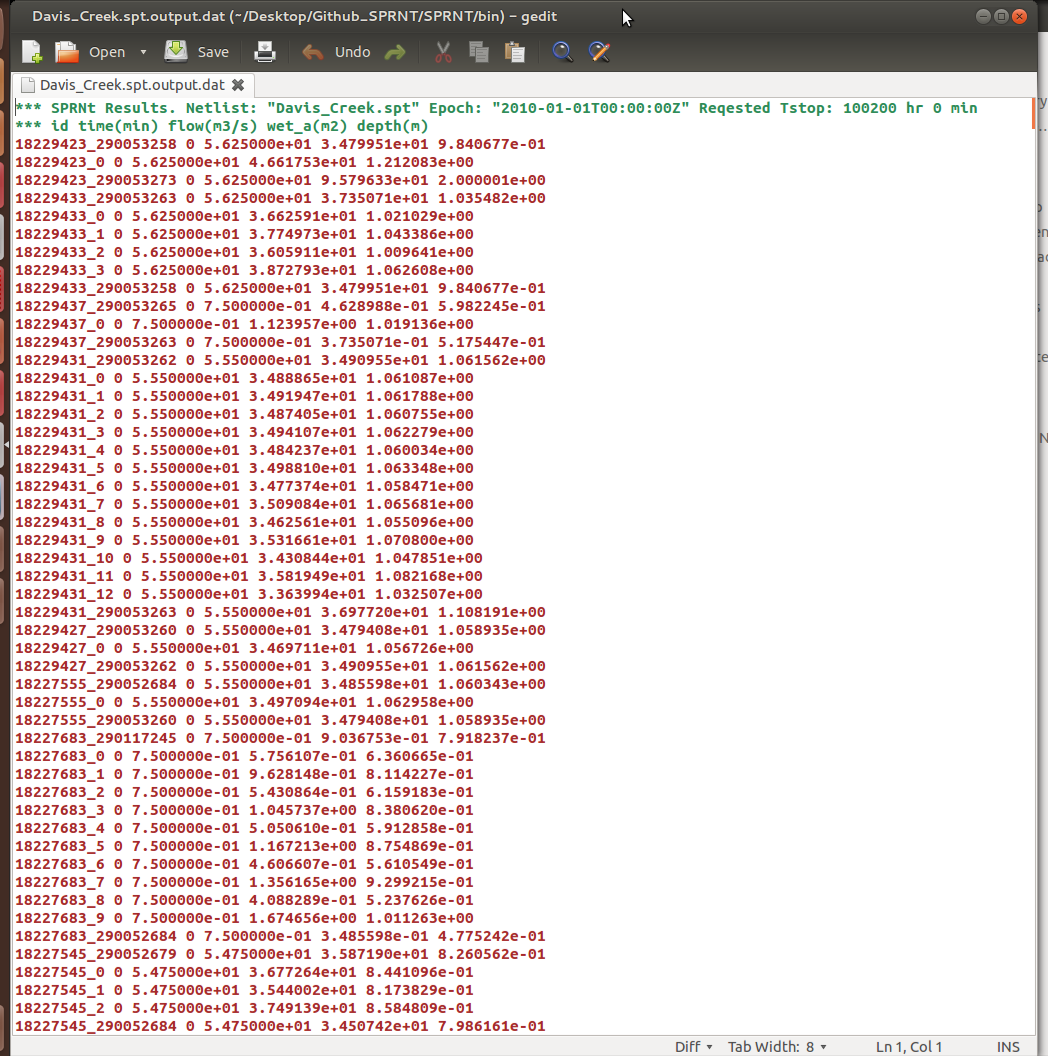
\includegraphics[width = 0.75\textwidth]{figure/outputfileformat.png} %
	\label{fig:process}%
\end{figure}

\subsection{``Checkonly" Mode in SPRNT}
In here, SPRNT also provides a ``Check-only" function for users to do quick topological check, which will print out the general information at each computation point, including Flowrate, Wetted Area, Water Depth and Froude number. This check mode can be executed by using the following command:
 
\begin{lstlisting}[frame=single]
$ sh run_spt.sh -checkonly FILENAME.spt
\end{lstlisting}

\newpage



\end{flushleft} %%End the left align

%%%%%%%%%%%%
\section{FAQ for SPRNT}
\begin{flushleft} %%Start Left align
In this section, some frequently asked questions and common error messages are listed for users reference. Every effort has been made to make this FAQ as informative as possible; if you have any suggestions as to how it may be improved, send them to Cheng-Wei Yu (\url{yuchanway@utexas.edu}).
\begin{enumerate}
\item \textbf{\color{red}{[EE] Bummer: time step too small at time point XXX second.}}\\
This error message is caused by the oscillation of the numerical solution, which is known as ``Gibb`s phenomenon". Usually, Gibb`s phenomenon will occur before a huge, flashy and suddenly runoff event. There are several appropriate solutions for this problem, and the most useful one is applying a filter (ex. Gaussian filter, lowpass filter) to smooth the peak and approach to the real hydrograph.

\item \textbf{\color{red}{Bummer: wetted area specification in INTRINSIC x-section has to be monotonically increasing.}}\\
Before running a SPRNT simulation, SPRNT will do a simple topography and river geometry check. If the user uses the intrinsic cross section to describe the channel property, the wetted area should increase with the depth increase. If SPRNT finds any of the channel properties violate this law, it will show this error message.

\item \textbf{\color{red}{[EE]: first phase of steady-state solve failed.}}\\
There are several possibilities to cause the steady state convergence failure, the most common one is the missetting of boundary conditions (ex. downstream boundary or contribution ratio in the junction).

\item \textbf{\color{red}{[EE]: second phase of steady state solve failed.}}\\
The reason to have this error message is similar to the ``first phase steady state solve failed". Once have this error message, please check your boundary conditions and other settings.

\item \textbf{\color{red}{DBINTK error}}\\
This message only shows when you have over-flat channel sidewalls. Since SPRNT is a one-dimensional hydrodynamic model, there are some limitations for the channel sidewall slope. The minimum sidewall slope value that SPRNT can take is 0.0015 (this value can vary due to different channel characteristics), once the channel sidewall slope is too flat, the flow in this channel section in the simulation will become a two-dimensional problem, which cannot be solved by SPRNT model.

\item \textbf{\color{red}{Bummer: error reading 4D data specified in line XX, requires at least 5 points.}}\\
The default requirement for an intrinsic cross section is 5 sets (A, P, Y, W) of data. If the given cross section data is less than 5 sets, SPRNT model will not be bale to build a complete cross section shape.

\item \textbf{\color{red}{== tchk == node ``XXXX\_XXXX" requires upstreaming Q.}}\\
The upstream forcing term cannot be set to 0. \newline
Unlike hydrological models, the upstream boundary flows can not be set to 0 in hydrodynamic models due to the necessity of initial state  and prevention of singularity matrices in numerical simulation. 

\item \textbf{\color{red}{== tchk == node ``XXXX\_XXXX" no flow path to downstream.}}\\
Two common reasons to have this error message. (1) Unbalance contribution ratios in the junction point. When there is a great difference between two inflow upstream in the junction point, flow from the minor upstream will be blocked and the flowline will be regarded as ``no flow path". For this case, users need to check if contribution ratios in junction are reasonable. (2) Unreasonable channel cross section combination. Overall, in natural rivers, the area of river bathymetry will gradually increase with the cumulative catchment area/flowrate, and this rule also applies to SPRNT model cross section setting. When users use the unreasonable cross section setting, for instance, wide upstream and narrow-shallow downstream, this error message will be triggered.  

\end{enumerate}
\end{flushleft} %%End left align
\newpage


%%%%%%%%%%%%%
\begin{appendices}
\section{How to use the Preprocessor}
\label{sec:HtuP}
\begin{flushleft} %%Begin left align

In here, we provided a ready-to-use data preprocessor for users' convenience to make a proper netlist files for running SPRNT model. 
In this section, we will go through every step of how to set up the simulation variables such as upstream/downstream boundary conditions, computational time-steps, result print time steps, and output filename in this ready-to-use preprocessor. \newline
\newline
\emph{[NOTE]: Mac users may need to install NetCDF library through Xcode when compiling the source code of this preprocessor, detailed tutorial about installing NetCDF on Mac machine can be found on the Internet.}

%%
\subsection*{Set up output filename and simulation time}
In the preprocessor directory, users can easily find a file called \emph{``tt.C"}, which is the environmental variables set up file of the SPRNT model. \emph{tt.C} also contains the main function of the preprocessor. \newline 
In this file, we will be able to configure the output filename (the *.spt file that we will use for running SPRNT), the steady state result filename, the length of simulation time, the length of computational time steps, and the printing interval in the SPRNT result file. The following picture is the screen snapshot of tt.c. 

\begin{figure}[H]
	\centering
	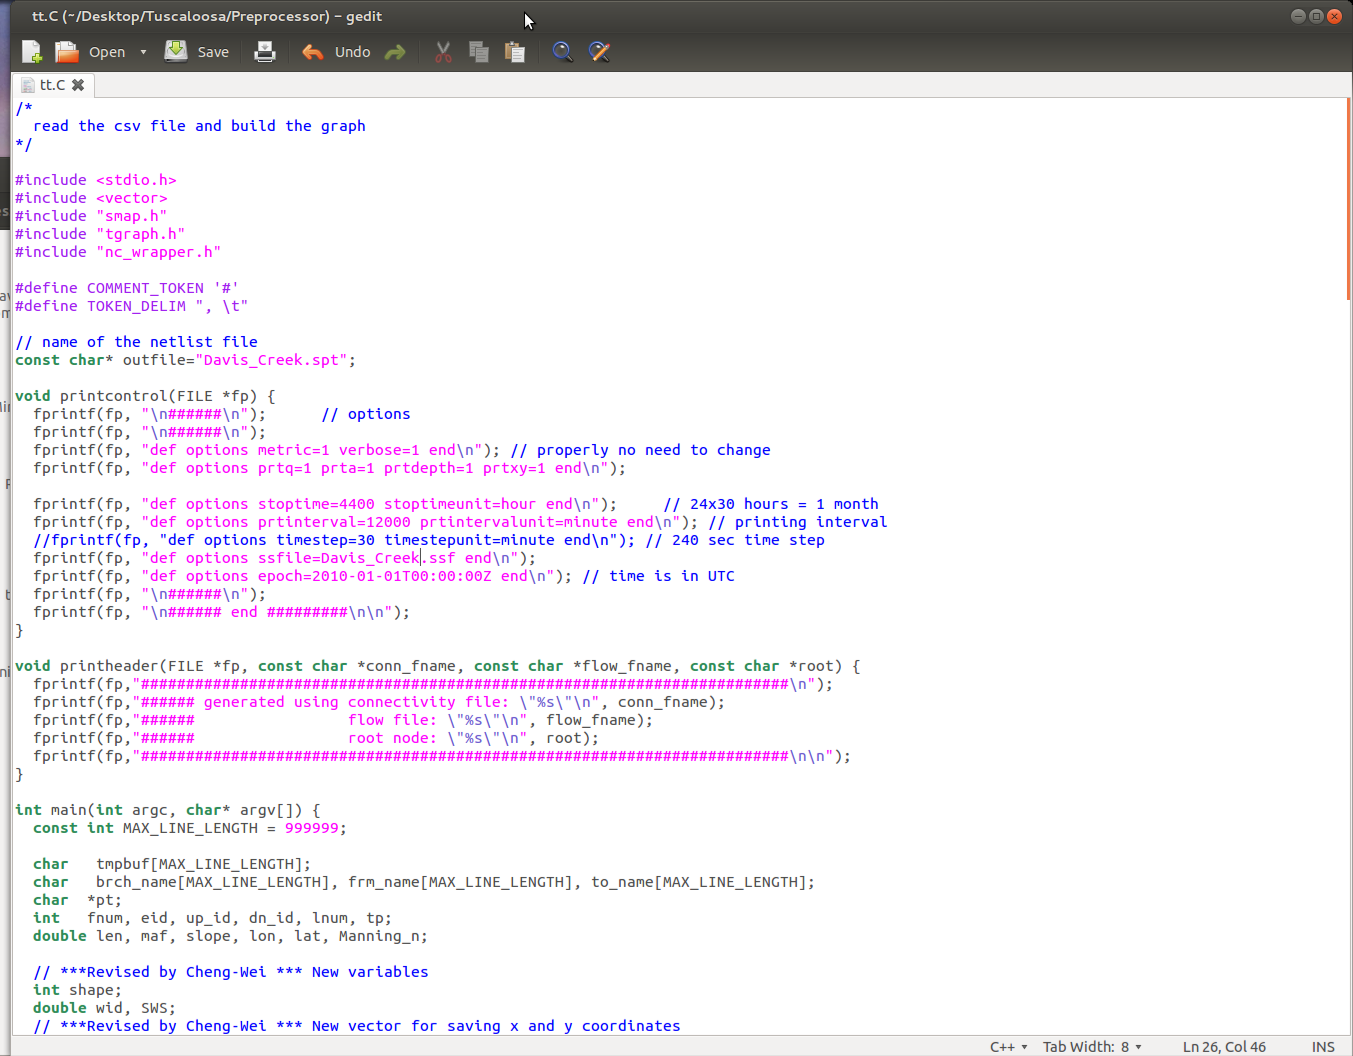
\includegraphics[width = 0.75\textwidth]{figure/tt.png} %
	\label{fig:process}%
\end{figure}

\lstset{language=C++,
                basicstyle=\ttfamily,
                keywordstyle=\color{blue}\ttfamily,
                stringstyle=\color{magenta}\ttfamily,
                commentstyle=\color{green}\ttfamily,
                morecomment=[l][\color{magenta}]{\#}
}
\newpage
\lstset{showstringspaces=false}
\begin{lstlisting}[frame=single]
char* outfile = "Davis_Creek.spt"
\end{lstlisting}

The ``Davis\_Creek.spt" here is the output filename you will produce from the preprocessor. It can be changed to any name end with .spt.
\newline
\lstset{language=C++,
                basicstyle=\ttfamily,
                keywordstyle=\color{blue}\ttfamily,
                stringstyle=\color{magenta}\ttfamily,
                commentstyle=\color{green}\ttfamily,
                morecomment=[l][\color{magenta}]{\#}
}
\lstset{showstringspaces=false}
\begin{lstlisting}[frame=single,basicstyle=\small]
fprintf(fp, "def options stoptime=4400 stoptimeunit=hour end\n"
\end{lstlisting}

The total length of simulation time can be set up in the above code line, in the example shown here, the simulation length is 4400 hours, which is about half year time. Please be aware of that the total simulation time should correspond to the time series you have in the \emph{Runoff NetCDF file}, or it can be shorter if users just need to simulate a particular time period. 
\newline
\lstset{language=C++,
                basicstyle=\ttfamily,
                keywordstyle=\color{blue}\ttfamily,
                stringstyle=\color{magenta}\ttfamily,
                commentstyle=\color{green}\ttfamily,
                morecomment=[l][\color{magenta}]{\#}
}
\lstset{showstringspaces=false}

\begin{lstlisting}[frame=single,basicstyle=\footnotesize]
fprintf(fp, "def options prtinterval=12000 prtintervalunit=minute end\n");
\end{lstlisting}

The command line here can control the printing interval in the result file, which is a ``*.spt.output.dat" file (users can go to section \textbf{``3.9 Result file structure"} for more details). Please notice that the printing interval unit is minutes. Since the default runoff time step from land surface model is normally hourly, the author suggests that the printing interval should be no shorter than 60 minutes. The finer of the printing interval, the bigger result file you will have. Sometimes the result file will up to $>$ 100GB when simulating a long simulation with fine printing intervals. 
The oversized output file will enhance the difficulty for users to open/read the result in the file, so choosing optimal printing interval wisely is a crucial task for users to decide.
%%%%
\newline
\lstset{language=C++,
                basicstyle=\ttfamily,
                keywordstyle=\color{blue}\ttfamily,
                stringstyle=\color{magenta}\ttfamily,
                commentstyle=\color{green}\ttfamily,
                morecomment=[l][\color{magenta}]{\#}
}
\lstset{showstringspaces=false}

\begin{lstlisting}[frame=single,basicstyle=\small]
fprintf(fp, "def options timestep=30 timestepunit=minute end\n");
\end{lstlisting}

This code line decides the length of computation time steps in the SPRNT model. However, the convergence stability of fixed length computational timestep in the finite difference method has been addressed in numbers of articles. %\add{[Need Cite articles]} 
Users need to use caution when setting a fixed computational timestep in this line. 
Fortunately, the SPRNT model provides a dynamic time step function, which can adjust the computational length automatically. If users want the SPRNT use the dynamic timestep function, just simply comment out this line (by adding ``//" at the beginning of the line).
%%%%
\newline
\lstset{language=C++,
                basicstyle=\ttfamily,
                keywordstyle=\color{blue}\ttfamily,
                stringstyle=\color{magenta}\ttfamily,
                commentstyle=\color{green}\ttfamily,
                morecomment=[l][\color{magenta}]{\#}
		}
\lstset{showstringspaces=false}
\begin{lstlisting}[frame=single]
fprintf(fp, "def options ssfile=Davis_Creek.ssf end\n");
\end{lstlisting}
In the SPRNT model, the steady state simulation will be solved before solving unsteady state computation. The result of the steady state will be saved in a `` *.ssf " file and used as the initial condition of unsteady state computation. In here, we use \textbf{Davis\_Creek.ssf} as an example.
\newline
\emph{[NOTE]: *.ssf is a text-base file for temporary data storage, and it is not a well-formatted output file for recording results. Users can disregard the contents of the *.ssf file.}
%%%%
\newline
\lstset{language=C++,
                basicstyle=\ttfamily,
                keywordstyle=\color{blue}\ttfamily,
                stringstyle=\color{magenta}\ttfamily,
                commentstyle=\color{green}\ttfamily,
                morecomment=[l][\color{magenta}]{\#}
		}
\lstset{showstringspaces=false}
\begin{lstlisting}[frame=single]
fprintf(fp, "def options epoch=2010-01-01T00:00:00Z end\n");
\end{lstlisting}
The starting UTC date and time (Users need to convert the time to appropriate time zone corresponds to the study area) of simulation can be set up here. The time setting here won't have any influence on the model result, it will only be printed in the header of the result file for users' reference.

\subsection*{Set up boundary conditions}
Boundary conditions can be defined in \emph{``tgraph.C"} file, which includes several different C++ classes to control the \emph{def - end} block printing in the netlist file. In this file, we will be able to define the downstream BC, upstream BC (forcing terms) and the length of spatial computational nodes.
\newline
\newline
At the top of the \emph{tgrapg.C} file, users can find the codes as shown in the following figure:
\begin{figure}[H]
	\centering
	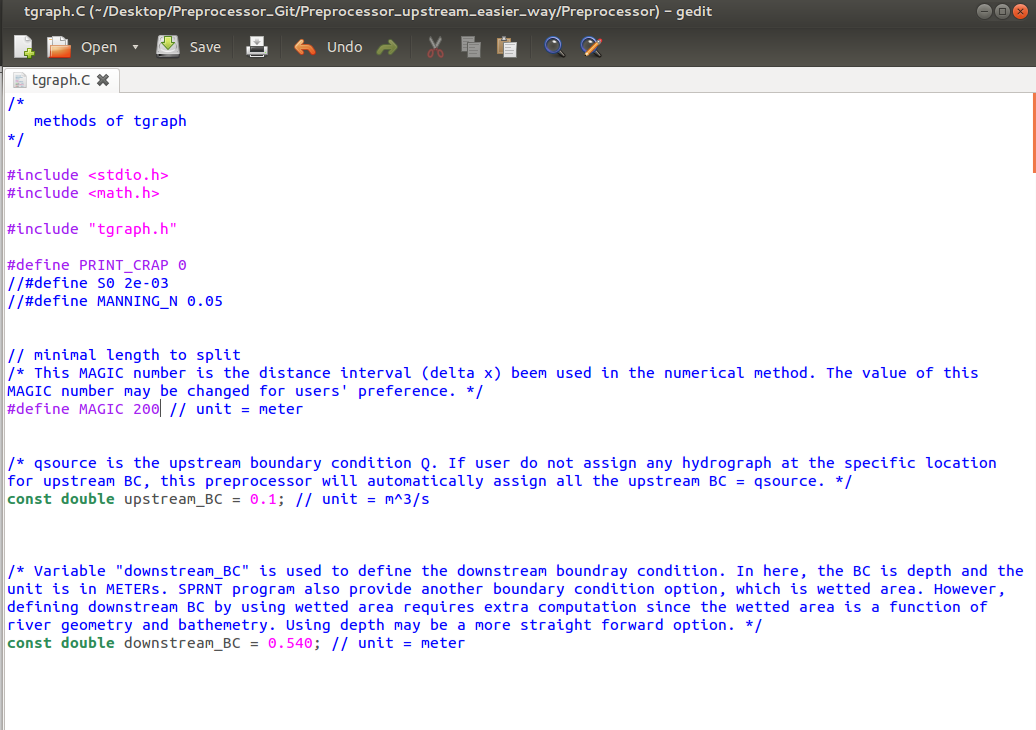
\includegraphics[width = 1.0\textwidth]{figure/tgraph.png} %
	\label{fig:process}%
\end{figure}
\newpage
In here, users can define boundary conditions and spatial length of computational nodes. Detailed instructions are elaborated in the following:
\newline
\newline
\textbf{Spatial interval of computational node}
\lstset{language=C++,
                basicstyle=\ttfamily,
                keywordstyle=\color{blue}\ttfamily,
                stringstyle=\color{magenta}\ttfamily,
                commentstyle=\color{green}\ttfamily,
                morecomment=[l][\color{magenta}]{\#}
		}
\lstset{showstringspaces=false}
\begin{lstlisting}[frame=single]
#define MAGIC 200  
\end{lstlisting}
This code line defines the spatial length of the computational node in the river network. In here, we use 200 meters as an instance, which means every flowline longer than 200 meters will be divided into several segments and computational nodes will be inserted between segments. For the flowline is shorter than 200 meters, the preprocessor will define it as 200 meters.\newline
\emph{[NOTE]: When setting the spatial interval length, Courant stability condition need to be contemplated by users in order to get a stable numerical solution.}
\newline
\newline
\textbf{Upstream boundary condition (forcing term)}
\lstset{language=C++,
                basicstyle=\ttfamily,
                keywordstyle=\color{mygreen}\ttfamily,
                stringstyle=\color{magenta}\ttfamily,
                commentstyle=\color{green}\ttfamily,
                morecomment=[l][\color{magenta}]{\#}
		}
\lstset{showstringspaces=false}
\begin{lstlisting}[frame=single]
const double upstream_BC = 0.1;  
\end{lstlisting}
In hydraulic/hydrodynamic models, the upstream boundary conditions are required to create an initial solution to avoid St. Venant Equations become singular. Normally, upstream boundary conditions(forcing terms) are often referred as the river ``baseflow", which can be found from the public/private agent such as USGS website. Recommended value for forcing terms is between 0.02 $m^3/s$ to 0.1 $m^3/s$.
\newline
\newline
\textbf{Downstream boundary condition}
\lstset{language=C++,
                basicstyle=\ttfamily,
                keywordstyle=\color{mygreen}\ttfamily,
                stringstyle=\color{magenta}\ttfamily,
                commentstyle=\color{green}\ttfamily,
                morecomment=[l][\color{magenta}]{\#}
		}
\lstset{showstringspaces=false}
\begin{lstlisting}[frame=single]
const double downstream_BC = 0.540;  
\end{lstlisting}
For downstream boundary condition, users need to specify the water depth (in meters) for the outlet point of the river network. 



%First, open the \textbf{tgraph.C} file, and use search function to search ``def boundarycondition", then you will be able to see the code shown in the following snapshot:
%
%\begin{figure}[H]
%	\centering
%	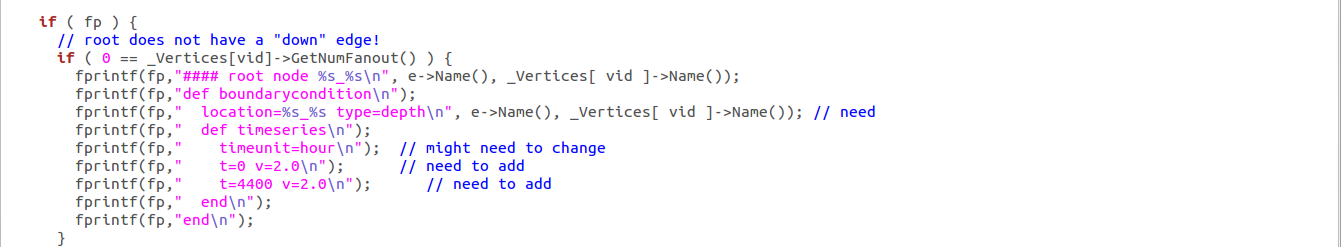
\includegraphics[width = 1.0\textwidth]{figure/tgraph_boundary.png} %
%	\label{fig:process}%
%\end{figure}
%This block defines the downstream boundary condition at the outlet node of your river network. The preprocess or will automatically define the location of the outlet node so there is no need to define it. What user need to change is the following lines:
%
%\lstset{language=C++,
%                basicstyle=\ttfamily,
%                keywordstyle=\color{blue}\ttfamily,
%                stringstyle=\color{magenta}\ttfamily,
%                commentstyle=\color{green}\ttfamily,
%                morecomment=[l][\color{magenta}]{\#}
%		}
%\lstset{showstringspaces=false}
%\begin{lstlisting}[frame=single]
%fprintf(fp,"	t=0 v=2.0\n"); 
%fprintf(fp,"	t=4400 v=2.0\n");
%\end{lstlisting}
%In this case, we define the start time and the end time downstream boundary conditions are both 2 m depth. If user want to add a changing point for the downstream boundary condition, you can simply add an extra line between the start time and the end time like this:
%
%
%
%\lstset{language=C++,
%                basicstyle=\ttfamily,
%                keywordstyle=\color{blue}\ttfamily,
%                stringstyle=\color{magenta}\ttfamily,
%                commentstyle=\color{green}\ttfamily,
%                morecomment=[l][\color{magenta}]{\#}
%		}
%\lstset{showstringspaces=false}
%\begin{lstlisting}[frame=single]
%printf(fp,"	t=0 v=2.0\n");
%printf(fp,"	t=1000 v=3.0\n");
%printf(fp,"	t=2000 v=2.5\n");
%printf(fp,"	t=4400 v=2.0\n");
%\end{lstlisting}
%
%After finish setting the downstream boundary condition, we need to set up the boundary condition on the upstream. Search ``def qsource" in tgraph.C, you will be able to see the lines in the following snapshot:
%
%
%\begin{figure}[H]
%	\centering
%	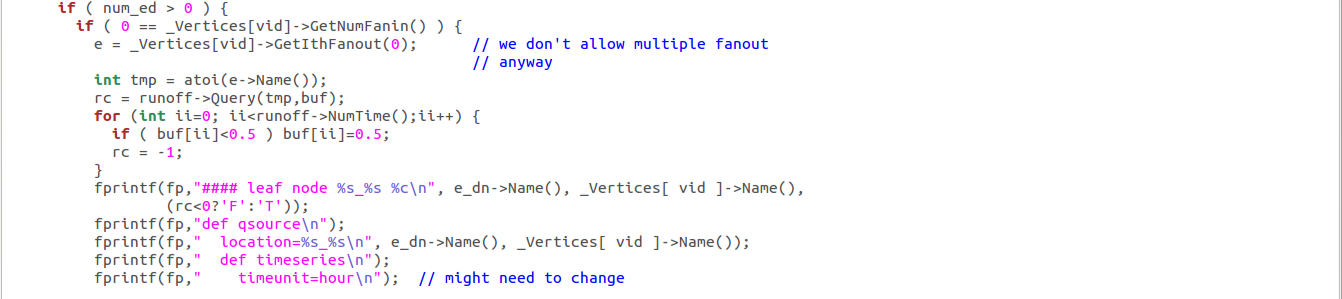
\includegraphics[width = 1.0\textwidth]{figure/tgraph_qsource.png} %
%	\label{fig:process}%
%\end{figure}
%
%The qsource block defines a Q source at the upstream pour-in point of the network. The Q source here is the forcing terms of the SPRNT model. These forcing terms provide an initial water level for solving the St. Venant Equations. The reason we need the forcing terms is that when there is no water flow in the channel, the St. Venant Equations become singular. Therefore, certain level of small flow is needed. Experimentally, a optimal qsource should between $0.02 m^3/s$ and $0.1 m^3/s$. Exceeding $0.5m3/s$ could influence the simulation result, especially the result at the downstream.
%To change the qsource, we can simply change the values in the following code line:
%\lstset{language=C++,
%                basicstyle=\ttfamily,
%                keywordstyle=\color{blue}\ttfamily,
%                stringstyle=\color{magenta}\ttfamily,
%                commentstyle=\color{green}\ttfamily,
%                morecomment=[l][\color{magenta}]{\#}
%		}
%\lstset{showstringspaces=false}
%\begin{lstlisting}[frame=single]
%if ( buf[ii]<0.5 ) buf[ii]=0.5;
%\end{lstlisting}
%
%In here , the qsource is set to be 0.5 m3/s. If user want to change it, for instance, 0.25, the code will become:
%
%\lstset{language=C++,
%                basicstyle=\ttfamily,
%                keywordstyle=\color{blue}\ttfamily,
%                stringstyle=\color{magenta}\ttfamily,
%                commentstyle=\color{green}\ttfamily,
%                morecomment=[l][\color{magenta}]{\#}
%		}
%\lstset{showstringspaces=false}
%\begin{lstlisting}[frame=single]
%if ( buf[ii]<0.25 ) buf[ii]=0.25;
%\end{lstlisting}
%
%It means that, the $0.25 m^/s$ initial flow will be poured in every upstream point. This initial flow can be regarded as the baseflow of the river. However, user should always be careful to decide a reasonable qsource value before running the simulation.

\subsection*{How to compile the preprocessor}
After setting up all the variables, users can compile the preprocessor by using following commands:
\begin{lstlisting}[frame=single]
$ make
\end{lstlisting}
\begin{figure}[H]
	\centering
	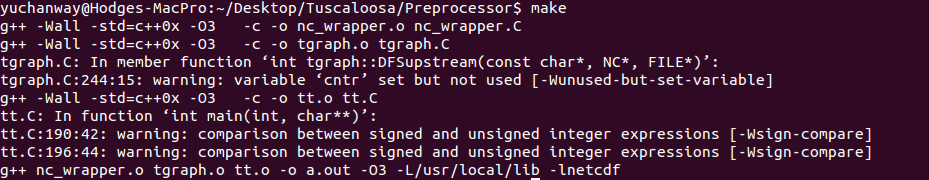
\includegraphics[width = 1.0\textwidth]{figure/make.png} %
	\label{fig:process}%
\end{figure}

After executing the \emph{"make"} command, users will see an executable file called \textbf{``a.out"} in the directory. This executable file is an assembler output file for connecting all the required codes/libraries to an executable code. Users can use this executable object to load the data in connectivity file and runoff NetCDF file by using the following commands:
\newline
\begin{lstlisting}[frame=single]
$ a.out Connectivity_filename.csv Runoff_NetCDF.nc
\end{lstlisting}
\begin{figure}[H]
	\centering
	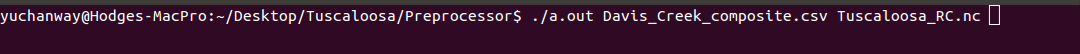
\includegraphics[width = 1.0\textwidth]{figure/aout_1.png} %
	\label{fig:process}%
\end{figure}
In this step, the preprocessor will scan all the data in the connectivity file(*.csv) and runoff NetCDF file(*.nc), to verify that the topography data matches the runoff data. Once the examination is done, the preprocessor will return the number of river network system in the study area by denoting the outlet point ``ToNode":

\begin{figure}[H]
	\centering
	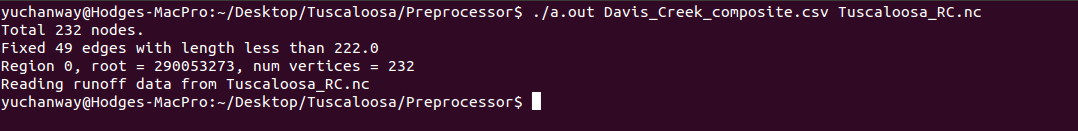
\includegraphics[width = 1.0\textwidth]{figure/aout_2.png} %
	\label{fig:process}%
\end{figure}

In our example here, we have only one river network in the Davis\_Creek\_composite.csv connectivity file, with outlet point ``290053273". If user wants to proceed to produce the netlist file, further command is required:

\begin{lstlisting}[frame=single,basicstyle=\small]
$ a.out Connectivity_filename.csv Runoff_NetCDF.nc Node_Number
\end{lstlisting}


\begin{figure}[H]
	\centering
	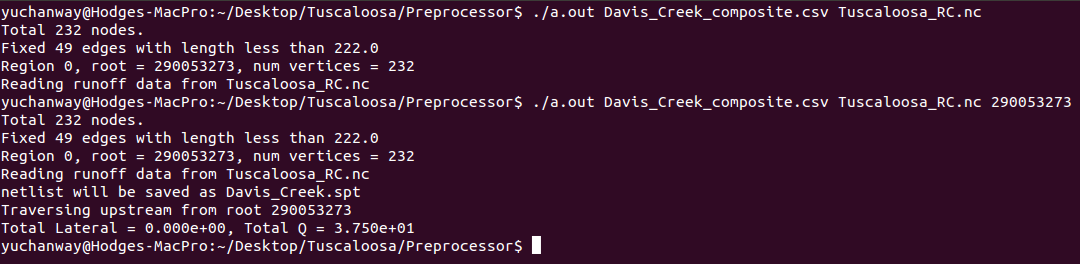
\includegraphics[width = 1.0\textwidth]{figure/aout_4.png} %
	\label{fig:process}%
\end{figure}


After executing above commands, the preprocessor will start to discard useless data (if there are other networks in the connectivity file) and extract the designate river network to produce the netlist file(*.spt). The final netlist filename will be the name that users setup in the \textbf{``tt.C"} file.
\newline
\newline
The final netlist file will be moved to the bin directory in SPRNT folder for running the simulation.
%
%\begin{lstlisting}[frame=single]
%$ mv Netlist_Filename.spt /PATH/SPRNT/bin
%\end{lstlisting}
%
%\begin{figure}[H]
%	\centering
%	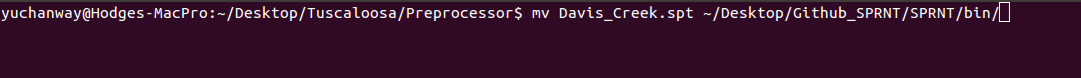
\includegraphics[width = 1.0\textwidth]{figure/mv_to_bin.png} %
%	\label{fig:process}%
%\end{figure}
%

\subsection*{Re-compile the preprocessor}

If there is any change in variables, please make sure to recompile the preprocessor by using the following two commands:

\begin{lstlisting}[frame=single]
$ make clean
\end{lstlisting}


\begin{lstlisting}[frame=single]
$ make realclean
\end{lstlisting}

These two commands will clean up all the old executable objects and dependency files. After setting up the new conditions/variables, remember to do the \textbf{``make"} command again to create a new executable object.

\end{flushleft} %%End left align

%
%\newpage
%\section{Pseudo unsteady method (Optional)}
%Pseudo unsteady method is a function that can be used to run a quasi-steady simulation to get the water surface elevation. By using this function with the peak flood value at each reach, users will be able to get the water surface elevation during the major flood event. Although this method was originally implemented to compute a consistent set of initial conditions for all nodes.and was not exposed to end-users, users still be able to use this function to get hydraulic simulation results by using some tricky settings. 
%
%Users can follow the following instructions:
%
%\begin{enumerate}
%\item Unlike to normal unsteady simulation, the runoff value here should be time-varying, but constant values (which is the peak value of the flood event at each reach location).
%\item Set the simulation time to a small value (ex. \emph{stoptime = 0.5}) in \textbf{tt.C} file (If you don't know where to find tt.C file, please go to Appendix \ref{sec:HtuP} for more information).
%\begin{lstlisting}[frame=single,basicstyle=\small]
%fprintf(fp, "def options stoptime=0.5 stoptimeunit=hour end\n"
%\end{lstlisting}
%
%\begin{figure}[H]
%	\centering
%	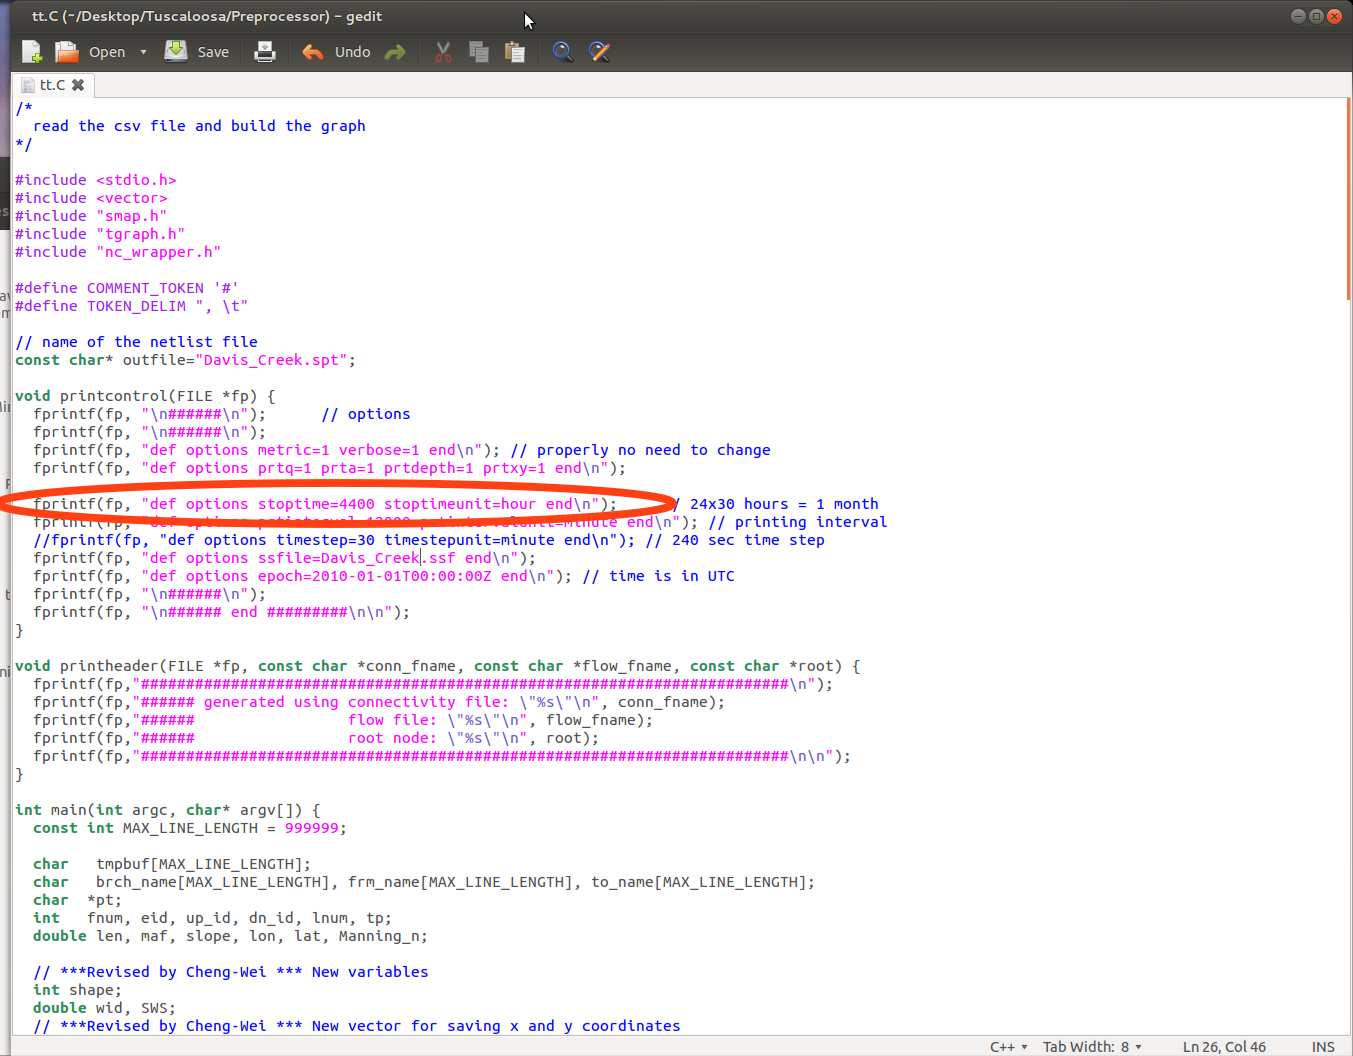
\includegraphics[width = 1.0\textwidth]{figure/pusedo.png} %
%	\label{fig:process}%
%\end{figure}
%
%\item For the other boundary conditions and forcing terms, just use the normal setting.
%\end{enumerate}
%
%The concept of this method is letting SPRNT to run a short time unsteady solve. When the SPRNT model execute the simulation, it will read in the constant runoff value and use it to run a quasi-steady solve. In the output file (\emph{NAME.spt.output.dat}), users can find the quasi-steady simulation result by using flood peak value (ex. flowrate, water surface elevation, wetted area).
%

\end{appendices}



\end{document}
%end
